% Этот шаблон документа разработан в 2014 году
% Данилом Фёдоровых (danil@fedorovykh.ru) 
% для использования в курсе 
% <<Документы и презентации в \LaTeX>>, записанном НИУ ВШЭ
% для Coursera.org: http://coursera.org/course/latex .
% Исходная версия шаблона --- 
% https://www.writelatex.com/coursera/latex/2

\documentclass[a4paper,12pt]{article}

%%% Работа с русским языком
\usepackage{cmap}					% поиск в PDF
\usepackage{mathtext} 				% русские буквы в формулах
\usepackage[T2A]{fontenc}			% кодировка
\usepackage[utf8]{inputenc}			% кодировка исходного текста
\usepackage[english,russian]{babel}	% локализация и переносы
\usepackage{xcolor} % управляем цветами текста и фона текста

\usepackage[most]{tcolorbox} % для управления цветом
\definecolor{block-gray}{gray}{0.90} % уровень прозрачности (1 - максимум)
\newtcolorbox{myquote}{colback=block-gray,grow to right by=-10mm,grow to left by=-10mm,
	boxrule=0pt,boxsep=0pt,breakable} % настройки области с изменённым фоном
%%% Дополнительная работа с математикой
\usepackage{amsfonts,amssymb,amsthm,mathtools} % AMS
\usepackage{amsmath}
\usepackage{icomma} % "Умная" запятая: $0,2$ --- число, $0, 2$ --- перечисление

%% Номера формул
%\mathtoolsset{showonlyrefs=true} % Показывать номера только у тех формул, на которые есть \eqref{} в тексте.

%% Шрифты
\usepackage{euscript}	 % Шрифт Евклид
\usepackage{mathrsfs} % Красивый матшрифт

%% Свои команды
\DeclareMathOperator{\sgn}{\mathop{sgn}}

%% Перенос знаков в формулах (по Львовскому)
\newcommand*{\hm}[1]{#1\nobreak\discretionary{}
{\hbox{$\mathsurround=0pt #1$}}{}}

%%% Работа с картинками
\usepackage{graphicx}  % Для вставки рисунков
\graphicspath{{images/}{images2/}}  % папки с картинками
\setlength\fboxsep{3pt} % Отступ рамки \fbox{} от рисунка
\setlength\fboxrule{1pt} % Толщина линий рамки \fbox{}
\usepackage{wrapfig} % Обтекание рисунков и таблиц текстом

%%% Работа с таблицами
\usepackage{array,tabularx,tabulary,booktabs} % Дополнительная работа с таблицами
\usepackage{longtable}  % Длинные таблицы
\usepackage{multirow} % Слияние строк в таблице
% в преамбуле
\usepackage[left=2cm,right=2cm,
top=2cm,bottom=2cm,bindingoffset=0cm]{geometry}



\begin{document} % конец преамбулы, начало документа


\newpage
\section{ER-диаграмма}
\begin{figure}[h]
	\center{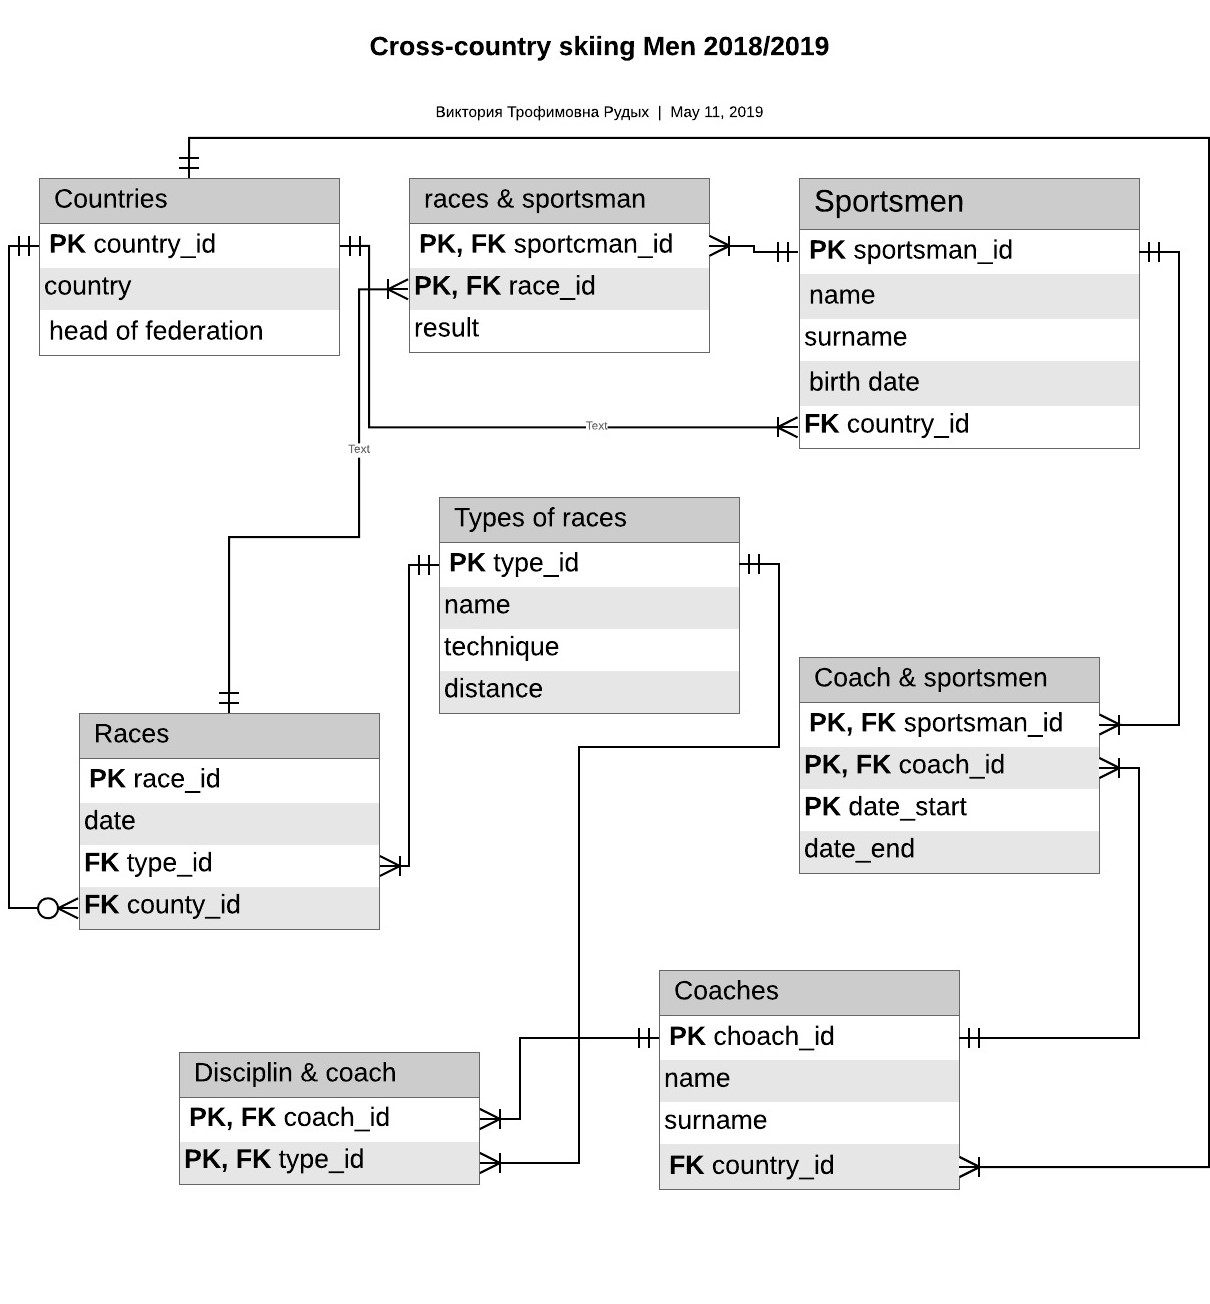
\includegraphics[width=\textwidth]{1.jpeg}}
\end{figure}
\section{Описание базы данных}

\noindent
\textbf{Cross-country skiing Men 2018/2019:} База данных состоит из 8 таблиц, в третьей нормальной форме. Описывает лыжние гонки 2018/2019 сезона. Содержит информацию о спортсменах, гонках, странах, тренерах и дисциплинах.\\
\textbf{Sportsmen:} Таблица, описывающая спортсменов. \textbf{PK} - sportsman\_id. Описание спортсмена - его имя, фамилия, дата рождения, страна.\\
\textbf{Counties:} Таблица, описывающая страны. \textbf{PK} - countries\_id. Описание страны - название страны, ФИ главы федерации.\\
\textbf{Races:} Таблица, описывающая гонки. \textbf{PK} - race\_id. Описание гонки - дата проведения гонки, тип гонки, страна проведения.\\
\textbf{Coaches:} Таблица, описывающая тренеров. \textbf{PK} - coach\_id. Описание тренера - его имя, фамилия, страна.\\
\textbf{Races \& sportsman:} Таблица, описывающая связь спортсменов с гонками, т. е. в какой гонке кто участвовал, и сколько баллов при этом набрал. \textbf{PK} - sportsman\_id, race\_id.\\
\textbf{Types of races:} Таблица, описывающая виды гонок. \textbf{PK} - type\_id. Описание типа гонок - название дисциплины, техника передвижения(классический стиль, коньковый стиль), дистанция.\\
\textbf{Disciplin \& coach:} Таблица, показывающая связь тренеров и дисциплин, т. е. какой тренер готовит к каким видам гонок. \textbf{PK} - type\_id, coach\_id.\\
\textbf{Coach \& sportsmen:} Таблица, описывающая связь тренеров и спортсменов, т. е. какой тренер тренирует какого спортсмена. Таблица является версионной SCD2, т. е. спортсмен может менять тренера за время карьеры. \textbf{PK} - coach\_id, sportsman\_id, date\_start. 

\section{Представления}
\textbf{Задание:} Написать 3-4 осмысленных представления, которые должны скрывать технические поля, или собирать и агрегировать данные из нескольких таблиц.\\ \\
\noindent
Разница между представленияеми и таблицами базы данных в том, что во всех таблицах связей используются суррогатные ключи, что неинформативнно для обычного пользвателя.\\
\textbf{Sportsmen:} Представление таблицы спортсменов, в котором выводится фамилия, имя, страна.\\
\noindent
\textbf{Races:} Представление гонок со странами и дистанцией, в котором выводится дата гонки, тип гонки, дистанция, страна проведения.\\
\noindent
\textbf{Races\_Sportsman:} Представление гонок со спортсменами и результами, в котором выводится фамилия спортсмена, дата гонки, результат.

\section{Тригеры и хранимые функции}
\textbf{Задание:} Написать не менее 2 хранимых процедур и не менее 2 тригеров.\\ \\
\textbf{age\_sp:} Функция определяет возраст спортсмена. Отдаем в нее дату рождения спортсмена, и функция вычисляет сколько лет прошло с этого момента до текущего момента.\\ \\
\textbf{before\_delete:} При удаление спортсмена проверяет, не остался ли он последним в своей стране. Если да, то бросает исключение. \\ \\
\textbf{Тригер - monitor\_sportsmen:} Используется для наблюдения за изменениеми в таблице спортсменов. При удалении/добавлении/обновлении вызывает вспомогательную функцию, которая во вспомогательную таблицу логов вносит строчку add/delete/update и sportsman\_id.\\

\section{Роли доступа}
\textbf{Задание:} Создать роли доступа и выдать права.\\ \\
\textbf{Обычный пользователь - ordinary\_user:} Может делать select, чтобы просматривать все таблицы.\\ \\
\textbf{Редактоp - editor:} Может работать с таблицами гонок, гонок и спортсменов, тренеров, дисциплин и тренеров, т. к. гонки и тренера - часто меняющиеся таблицыю. Может делать delete/update/insert в эти таблицы.\\\\\
\textbf{Модератор - moderator:} Может работать со всеми таблицами, т. е. делать delete/update/insert во все таблицы. \\\\
\textbf{Администратор - administrator:} Может работать со всеми таблицами, а также выдавать права на delete/update/insert другим пользователям.
\newpage
\section{Приложение}
create schema cross\_country\_skiing;\\
\\
create type \_tech as enum ('C', 'K', 'Both');\\
create type \_result as enum ('1', '2', '3');\\
\\
CREATE TABLE cross\_country\_skiing.countries(\\
\indent country\_id SERIAL PRIMARY KEY,\\
\indent country VARCHAR(30) NOT NULL UNIQUE,\\
\indent head\_of\_federation varchar(30)\\
);\\
\\
create table cross\_country\_skiing.types\_of\_races(\\
\indent type\_id serial primary key,\\
\indent name varchar(30) not null,\\
\indent technique \_tech,\\
\indent distance integer\\
);\\
\\
create table cross\_country\_skiing.races (\\
\indent race\_id serial primary key,\\
\indent date date,\\
\indent type\_id serial not null,\\
\indent country\_id serial not null,\\
\indent foreign key (country\_id)\\
\indent \indent references cross\_country\_skiing.countries(country\_id),\\
\indent foreign key (type\_id)\\
\indent \indent references cross\_country\_skiing.types\_of\_races(type\_id)\\
);\\
\\
create table cross\_country\_skiing.sportsmen (\\
\indent sportsman\_id serial primary key,\\
\indent name varchar(30) not null,\\
\indent surname varchar(30) not null unique,\\
\indent birth\_date date,\\
\indent country\_id serial not null,\\
\indent foreign key (country\_id)\\
\indent \indent references cross\_country\_skiing.countries(country\_id)\\
);\\
\\
create table cross\_country\_skiing.sportsman\_race(\\
\indent sportsman\_id serial not null,\\
\indent race\_id serial not null,\\
\indent result \_result,\\
\indent primary key(sportsman\_id,race\_id),\\
\indent foreign key(sportsman\_id)\\
\indent \indent references cross\_country\_skiing.sportsmen(sportsman\_id),\\
\indent foreign key(race\_id)\\
\indent \indent references cross\_country\_skiing.races(race\_id)\\
);\\
\\
create table cross\_country\_skiing.coaches(\\
\indent coach\_id serial primary key,\\
\indent name varchar(30) not null,\\
\indent surname varchar(30) not null unique,\\
\indent country\_id serial not null,\\
\indent foreign key(country\_id)\\
\indent \indent references cross\_country\_skiing.countries(country\_id)\\
);\\
\\
create table cross\_country\_skiing.coach\_sportsman(\\
\indent sportsman\_id SERIAL NOT NULL,\\
\indent coach\_id SERIAL NOT NULL,\\
\indent date\_start smallint not null,\\
\indent date\_end smallint not null,\\
\indent PRIMARY KEY (sportsman\_id, coach\_id, date\_start),\\
\indent FOREIGN KEY (sportsman\_id)\\
\indent \indent REFERENCES cross\_country\_skiing.sportsmen(sportsman\_id),\\
\indent FOREIGN KEY (coach\_id)\\
\indent \indent REFERENCES cross\_country\_skiing.coaches(coach\_id)\\
);\\
\\
create table cross\_country\_skiing.discipline\_coach(\\
\indent coach\_id SERIAL NOT NULL,\\
\indent type\_id SERIAL NOT NULL,\\
\indent PRIMARY KEY (coach\_id, type\_id),\\
\indent FOREIGN KEY (coach\_id)\\
\indent \indent REFERENCES cross\_country\_skiing.coaches(coach\_id),\\
\indent FOREIGN KEY (type\_id)\\
\indent \indent REFERENCES cross\_country\_skiing.types\_of\_races(type\_id)\\
);\\
\\
-- Функция определяющая возраст спортсмена, в конце есть пример использования\\
create or replace function age\_sp(birth\_date date)\\
returns int\\
as \$\$\\
declare i int := 0;\\
begin\\
\indent while birth\_date < now()\\
\indent loop\\
\indent \indent birth\_date := birth\_date + interval '1 year';\\
\indent \indent i := i + 1;\\
\indent end loop;\\
\indent return i;\\
end;\\
\$\$ language plpgsql;\\
\\
-- Таблица для тригера\\
CREATE TABLE cross\_country\_skiing.logs\\
(\\
\indent operation\_id serial not null,\\
\indent "info" varchar(100),\\
\indent "time" timestamp(0) without time zone\\
);\\
\\
-- Функция для тригера\\
CREATE OR REPLACE FUNCTION add\_to\_log() RETURNS TRIGGER AS \$\$\\
DECLARE\\
\indent mess varchar(100);\\
\indent sp\_id varchar(100);\\
\indent final varchar(254);\\
BEGIN\\
\indent IF  TG\_OP = 'INSERT' THEN\\
\indent \indent sp\_id = NEW.sportsman\_id;\\
\indent \indent mess := 'Added new sportsmen with sportsmen\_id = ';\\
\indent \indent final := mess || sp\_id;\\
\indent \indent INSERT INTO cross\_country\_skiing.logs values (default, final, NOW());\\
\indent \indent RETURN NEW;\\
\indent ELSIF TG\_OP = 'UPDATE' THEN\\
\indent \indent sp\_id = NEW.sportsman\_id;\\
\indent \indent mess := 'Updated sportsmen with sportsmen\_id ';\\
\indent \indent final := mess || sp\_id;\\
\indent \indent INSERT INTO cross\_country\_skiing.logs values (default, final, NOW());\\
\indent \indent RETURN NEW;\\
\indent ELSIF TG\_OP = 'DELETE' THEN\\
\indent \indent sp\_id = OLD.sportsman\_id;\\
\indent \indent mess := 'Removed user with sportsmen\_id';\\
\indent \indent final := mess || sp\_id;\\
\indent \indent INSERT INTO cross\_country\_skiing.logs values (default, final, NOW());\\
\indent \indent RETURN OLD;\\
\indent END IF;\\
END;\\
\$\$ LANGUAGE plpgsql;\\
\\
CREATE TRIGGER monitor\_sportsmen\\
AFTER INSERT OR UPDATE or delete ON cross\_country\_skiing.sportsmen FOR EACH ROW EXECUTE PROCEDURE add\_to\_log ();\\
\\
-- Функция ограничение на удаление последнего спортсмена, тоже с тригером, чтобы она автоматически запускалась перед попытой удаления\\
CREATE OR REPLACE FUNCTION before\_delete() RETURNS TRIGGER AS \$\$\\
BEGIN\\
\indent if exists (select count(cross\_country\_skiing.sportsmen.sportsman\_id) from cross\_country\_skiing.sportsmen\\
\indent \indent where cross\_country\_skiing.sportsmen.country\_id = new.country\_id\\
\indent \indent group by cross\_country\_skiing.sportsmen.country\_id\\
\indent \indent having count(cross\_country\_skiing.sportsmen.sportsman\_id) > 1)\\
\indent \indent then\\
\indent \indent begin\\
\indent \indent \indent return old;\\
\indent \indent end;\\
\indent else\\
\indent \indent raise exception 'Sportsman who you are trying to delete is the last from his country';\\
\indent end if;\\
END;\\
\$\$ LANGUAGE plpgsql;\\
\\
CREATE TRIGGER check\_remove\\
BEFORE delete ON cross\_country\_skiing.sportsmen FOR EACH ROW EXECUTE PROCEDURE before\_delete ();\\
\\
\\
insert into cross\_country\_skiing.countries values(default, 'Russia', 'Elena Vialbe');\\
insert into cross\_country\_skiing.countries values(default, 'Norway', 'Eric Roeste');\\
insert into cross\_country\_skiing.countries values(default, 'Finland',  'Markku Haapasalmi');\\
insert into cross\_country\_skiing.countries values(default, 'Italy',  'Loretta Piroia');\\
insert into cross\_country\_skiing.countries values(default, 'Swedish',  'Karin Weijber');\\
insert into cross\_country\_skiing.countries values(default, 'German', 'Alfons Hormann');\\
insert into cross\_country\_skiing.countries values(default, 'Khazakstan', 'Sorokin Vladimir');\\
insert into cross\_country\_skiing.countries values(default, 'USA',  'Simi Hamilton');\\
insert into cross\_country\_skiing.countries values(default, 'Canada', 'Tyler King');\\
insert into cross\_country\_skiing.countries values(default, 'Austria',  'Peter Schrocksnadel');\\
insert into cross\_country\_skiing.countries values(default, 'Switzeland', 'Gian-Franco Kasper');\\
insert into cross\_country\_skiing.countries values(default, 'France', 'Jan Kasper');\\
\\
insert into cross\_country\_skiing.types\_of\_races values (default, 'Skiatlon', 'Both',  '30');\\
insert into cross\_country\_skiing.types\_of\_races values (default, 'Sprint', 'C', '4');\\
insert into cross\_country\_skiing.types\_of\_races values (default, 'Sprint', 'K', '3');\\
insert into cross\_country\_skiing.types\_of\_races values (default, 'Individual race',  'C','15');\\
insert into cross\_country\_skiing.types\_of\_races values (default, 'Individual race',  'K', '10');\\
insert into cross\_country\_skiing.types\_of\_races values (default, 'Maraphon', 'C', '50');\\
insert into cross\_country\_skiing.types\_of\_races values (default, 'Maraphon', 'K', '40');\\
insert into cross\_country\_skiing.types\_of\_races values (default, 'Pursuit',  'C', '10');\\
insert into cross\_country\_skiing.types\_of\_races values (default, 'Pursuit',  'K', '15');\\
insert into cross\_country\_skiing.types\_of\_races values (default, 'Relay',  'C', '10');\\
insert into cross\_country\_skiing.types\_of\_races values (default, 'Relay',  'K', '10');\\
insert into cross\_country\_skiing.types\_of\_races values (default, 'Mass start', 'C', '15');\\
insert into cross\_country\_skiing.types\_of\_races values (default, 'Mass start', 'K', '10');\\
\\
\\
insert into cross\_country\_skiing.races values(default, '24.11.2018', '2', '3');\\
insert into cross\_country\_skiing.races values(default, '25.11.2018', '4', '3');\\
insert into cross\_country\_skiing.races values(default, '30.11.2018', '3', '2');\\
insert into cross\_country\_skiing.races values(default, '01.12.2018', '5', '2');\\
insert into cross\_country\_skiing.races values(default, '02.12.2018', '8', '2');\\
insert into cross\_country\_skiing.races values(default, '15.12.2018', '3', '4');\\
insert into cross\_country\_skiing.races values(default, '16.12.2018', '5', '4');\\
insert into cross\_country\_skiing.races values(default, '05.01.2019', '13',  '4');\\
insert into cross\_country\_skiing.races values(default, '12.01.2019', '2', '6');\\
insert into cross\_country\_skiing.races values(default, '13.01.2019', '6', '6');\\
insert into cross\_country\_skiing.races values(default, '09.02.2019', '1', '3');\\
insert into cross\_country\_skiing.races values(default, '10.02.2019', '7', '3');\\
insert into cross\_country\_skiing.races values(default, '27.02.2019', '4', '8');\\
insert into cross\_country\_skiing.races values(default, '01.03.2019', '10',  '8');\\
insert into cross\_country\_skiing.races values(default, '03.03.2019', '7', '8');\\
insert into cross\_country\_skiing.races values(default, '16.03.2019', '11',  '5');\\
insert into cross\_country\_skiing.races values(default, '22.03.2019', '12',  '9');\\
insert into cross\_country\_skiing.races values(default, '23.03.2019', '9', '9');\\
\\
\\
insert into cross\_country\_skiing.sportsmen values \\
\indent \indent \indent \indent \indent \indent \indent (default, 'Alexander', 'Bolshunov', '31.12.1996',  '1');\\
insert into cross\_country\_skiing.sportsmen values \\
\indent \indent \indent \indent \indent \indent \indent (default, 'Denis', 'Spitsov', '16.08.1996',  '1');\\
insert into cross\_country\_skiing.sportsmen values \\
\indent \indent \indent \indent \indent \indent \indent (default, 'Evgeniy', 'Belov', '07.08.1990',  '1');\\
insert into cross\_country\_skiing.sportsmen values \\
\indent \indent \indent \indent \indent \indent \indent (default, 'Sergey',  'Ustygov', '08.04.1992',  '1');\\
insert into cross\_country\_skiing.sportsmen values \\
\indent \indent \indent \indent \indent \indent \indent (default, 'Johanes', 'Klaebo',  '22.10.1996',  '2');\\
insert into cross\_country\_skiing.sportsmen values \\
\indent \indent \indent \indent \indent \indent \indent (default, 'Emil',  'Iversen', '12.08.1991',  '2');\\
insert into cross\_country\_skiing.sportsmen values \\
\indent \indent \indent \indent \indent \indent \indent (default, 'Sjir',  'Rothe', '02.07.1988',   '2');\\
insert into cross\_country\_skiing.sportsmen values \\
\indent \indent \indent \indent \indent \indent \indent (default, 'Simen', 'Kruger',  '13.03.1993',  '2');\\
insert into cross\_country\_skiing.sportsmen values \\
\indent \indent \indent \indent \indent \indent \indent (default, 'Martin',  'Sundby',  '26.09.1984',  '2');\\
insert into cross\_country\_skiing.sportsmen values \\
\indent \indent \indent \indent \indent \indent \indent (default, 'Janosh',  'Brugger', '01.06.1997',  '6');\\
insert into cross\_country\_skiing.sportsmen values \\
\indent \indent \indent \indent \indent \indent \indent (default, 'Federico',  'Pellegrino',  '01.09.1990',  '4');\\
insert into cross\_country\_skiing.sportsmen values \\
\indent \indent \indent \indent \indent \indent \indent (default, 'Francesco', 'De Fabiani',  '21.04.1993',  '4');\\
insert into cross\_country\_skiing.sportsmen values \\
\indent \indent \indent \indent \indent \indent \indent (default, 'Adrien',  'Backsheider', '07.08.1992',  '10');\\
insert into cross\_country\_skiing.sportsmen values \\
\indent \indent \indent \indent \indent \indent \indent (default, 'Moris', 'Manificat', '04.04.1986',  '10');\\
insert into cross\_country\_skiing.sportsmen values \\
\indent \indent \indent \indent \indent \indent \indent (default, 'Richard', 'Jouve', '25.10.1994',  '10');\\
insert into cross\_country\_skiing.sportsmen values \\
\indent \indent \indent \indent \indent \indent \indent (default, 'Jean',  'Gailard', '07.10.1980',  '10');\\
insert into cross\_country\_skiing.sportsmen values \\
\indent \indent \indent \indent \indent \indent \indent (default, 'Iivo',  'Niskanen',  '12.01.1992',  '3');\\
insert into cross\_country\_skiing.sportsmen values \\
\indent \indent \indent \indent \indent \indent \indent (default, 'Alex',  'Harvey',  '07.09.1988',  '8');\\
insert into cross\_country\_skiing.sportsmen values \\
\indent \indent \indent \indent \indent \indent \indent (default, 'Erik',  'Bjorsnen',  '14.07.1991',  '7');\\
insert into cross\_country\_skiing.sportsmen values \\
\indent \indent \indent \indent \indent \indent \indent (default, 'Calle', 'Halvarsson',  '17.03.1989',  '5');\\
insert into cross\_country\_skiing.sportsmen values \\
\indent \indent \indent \indent \indent \indent \indent (default, 'Dario', 'Cologna', '11.03.1986',  '9');\\
\\
insert into cross\_country\_skiing.sportsman\_race values('1',  '1', '1');\\
insert into cross\_country\_skiing.sportsman\_race values('5',  '1', '2');\\
insert into cross\_country\_skiing.sportsman\_race values('7',  '1', '3');\\
insert into cross\_country\_skiing.sportsman\_race values('1',  '2', '1');\\
insert into cross\_country\_skiing.sportsman\_race values('6',  '2', '2');\\
insert into cross\_country\_skiing.sportsman\_race values('20', '2', '3');\\
insert into cross\_country\_skiing.sportsman\_race values('11', '3', '1');\\
insert into cross\_country\_skiing.sportsman\_race values('6',  '3', '2');\\
insert into cross\_country\_skiing.sportsman\_race values('18', '3', '3');\\
insert into cross\_country\_skiing.sportsman\_race values('7',  '4', '1');\\
insert into cross\_country\_skiing.sportsman\_race values('8',  '4', '2');\\
insert into cross\_country\_skiing.sportsman\_race values('2',  '4', '3');\\
insert into cross\_country\_skiing.sportsman\_race values('10', '5', '1');\\
insert into cross\_country\_skiing.sportsman\_race values('16', '5', '2');\\
insert into cross\_country\_skiing.sportsman\_race values('19', '5', '3');\\
insert into cross\_country\_skiing.sportsman\_race values('5',  '6', '1');\\
insert into cross\_country\_skiing.sportsman\_race values('11', '6', '2');\\
insert into cross\_country\_skiing.sportsman\_race values('13', '6', '3');\\
insert into cross\_country\_skiing.sportsman\_race values('3',  '7', '1');\\
insert into cross\_country\_skiing.sportsman\_race values('14', '7', '2');\\
insert into cross\_country\_skiing.sportsman\_race values('9',  '7', '3');\\
insert into cross\_country\_skiing.sportsman\_race values('5',  '8', '1');\\
insert into cross\_country\_skiing.sportsman\_race values('12', '8', '2');\\
insert into cross\_country\_skiing.sportsman\_race values('1',  '8', '3');\\
insert into cross\_country\_skiing.sportsman\_race values('5',  '9', '1');\\
insert into cross\_country\_skiing.sportsman\_race values('4',  '9', '2');\\
insert into cross\_country\_skiing.sportsman\_race values('8',  '9', '3');\\
insert into cross\_country\_skiing.sportsman\_race values('21', '10',  '1');\\
insert into cross\_country\_skiing.sportsman\_race values('2',  '10',  '2');\\
insert into cross\_country\_skiing.sportsman\_race values('6',  '10',  '3');\\
insert into cross\_country\_skiing.sportsman\_race values('17', '11',  '1');\\
insert into cross\_country\_skiing.sportsman\_race values('10', '11',  '2');\\
insert into cross\_country\_skiing.sportsman\_race values('7',  '11',  '3');\\
insert into cross\_country\_skiing.sportsman\_race values('9',  '12',  '1');\\
insert into cross\_country\_skiing.sportsman\_race values('7',  '12',  '2');\\
insert into cross\_country\_skiing.sportsman\_race values('5',  '12',  '3');\\
insert into cross\_country\_skiing.sportsman\_race values('20', '13',  '1');\\
insert into cross\_country\_skiing.sportsman\_race values('1',  '13',  '2');\\
insert into cross\_country\_skiing.sportsman\_race values('6',  '13',  '3');\\
insert into cross\_country\_skiing.sportsman\_race values('5',  '15',  '1');\\
insert into cross\_country\_skiing.sportsman\_race values('11', '15',  '2');\\
insert into cross\_country\_skiing.sportsman\_race values('1',  '15',  '3');\\
insert into cross\_country\_skiing.sportsman\_race values('3',  '17',  '1');\\
insert into cross\_country\_skiing.sportsman\_race values('8',  '17',  '2');\\
insert into cross\_country\_skiing.sportsman\_race values('7',  '17',  '3');\\
insert into cross\_country\_skiing.sportsman\_race values('8',  '18',  '1');\\
insert into cross\_country\_skiing.sportsman\_race values('9',  '18',  '2');\\
insert into cross\_country\_skiing.sportsman\_race values('21', '18',  '3');\\
insert into cross\_country\_skiing.sportsman\_race values('5',  '14',  '1');\\
insert into cross\_country\_skiing.sportsman\_race values('6',  '14',  '1');\\
insert into cross\_country\_skiing.sportsman\_race values('7',  '14',  '1');\\
insert into cross\_country\_skiing.sportsman\_race values('9',  '14',  '1');\\
insert into cross\_country\_skiing.sportsman\_race values('1',  '14',  '2');\\
insert into cross\_country\_skiing.sportsman\_race values('2',  '14',  '2');\\
insert into cross\_country\_skiing.sportsman\_race values('3',  '14',  '2');\\
insert into cross\_country\_skiing.sportsman\_race values('4',  '14',  '2');\\
insert into cross\_country\_skiing.sportsman\_race values('13', '14',  '3');\\
insert into cross\_country\_skiing.sportsman\_race values('14', '14',  '3');\\
insert into cross\_country\_skiing.sportsman\_race values('15', '14',  '3');\\
insert into cross\_country\_skiing.sportsman\_race values('16', '14',  '3');\\
insert into cross\_country\_skiing.sportsman\_race values('1',  '16',  '1');\\
insert into cross\_country\_skiing.sportsman\_race values('2',  '16',  '1');\\
insert into cross\_country\_skiing.sportsman\_race values('3',  '16',  '1');\\
insert into cross\_country\_skiing.sportsman\_race values('4',  '16',  '1');\\
insert into cross\_country\_skiing.sportsman\_race values('5',  '16',  '2');\\
insert into cross\_country\_skiing.sportsman\_race values('6',  '16',  '2');\\
insert into cross\_country\_skiing.sportsman\_race values('7',  '16',  '2');\\
insert into cross\_country\_skiing.sportsman\_race values('8',  '16',  '2');\\
insert into cross\_country\_skiing.sportsman\_race values('13', '16',  '3');\\
insert into cross\_country\_skiing.sportsman\_race values('14', '16',  '3');\\
insert into cross\_country\_skiing.sportsman\_race values('15', '16',  '3');\\
insert into cross\_country\_skiing.sportsman\_race values('16', '16',  '3');\\
\\
insert into cross\_country\_skiing.coaches values (default, 'Marcus',  'Cramer',  '6');\\
insert into cross\_country\_skiing.coaches values (default, 'Uriy',  'Borodavko', '1');\\
insert into cross\_country\_skiing.coaches values (default, 'Arlid', 'Monser',  '2');\\
insert into cross\_country\_skiing.coaches values (default, 'Petter',  'Bransdal',  '2');\\
insert into cross\_country\_skiing.coaches values (default, 'Gury',  'Hetland', '2');\\
insert into cross\_country\_skiing.coaches values (default, 'Alonzo',  'Burgmaster',  '9');\\
insert into cross\_country\_skiing.coaches values (default, 'Doren', 'Aber',  '10');\\
insert into cross\_country\_skiing.coaches values (default, 'Kerty', 'Niskanen',  '3');\\
insert into cross\_country\_skiing.coaches values (default, 'Zibert',  'Clause',  '6');\\
insert into cross\_country\_skiing.coaches values (default, 'Martin',  'Weng',  '2');\\
insert into cross\_country\_skiing.coaches values (default, 'Sam', 'Wilson',  '8');\\
insert into cross\_country\_skiing.coaches values (default, 'Ricard',  'Grenborg',  '5');\\
insert into cross\_country\_skiing.coaches values (default, 'Yanne', 'Anderson',  '5');\\
\\
insert into cross\_country\_skiing.coach\_sportsman values ('4',  '1', '2002',  '3000');\\
insert into cross\_country\_skiing.coach\_sportsman values ('1',  '2', '2006',  '3000');\\
insert into cross\_country\_skiing.coach\_sportsman values ('2',  '1', '2002',  '3000');\\
insert into cross\_country\_skiing.coach\_sportsman values ('3',  '2', '2002',  '3000');\\
insert into cross\_country\_skiing.coach\_sportsman values ('5',  '3', '2002',  '3000');\\
insert into cross\_country\_skiing.coach\_sportsman values ('6',  '4', '2003',  '3000');\\
insert into cross\_country\_skiing.coach\_sportsman values ('7',  '4', '2004',  '3000');\\
insert into cross\_country\_skiing.coach\_sportsman values ('8',  '3', '2008',  '2016');\\
insert into cross\_country\_skiing.coach\_sportsman values ('7',  '3', '2017',  '3000');\\
insert into cross\_country\_skiing.coach\_sportsman values ('9',  '4', '2007',  '3000');\\
insert into cross\_country\_skiing.coach\_sportsman values ('10', '9', '2008',  '3000');\\
insert into cross\_country\_skiing.coach\_sportsman values ('11', '2', '2004',  '3000');\\
insert into cross\_country\_skiing.coach\_sportsman values ('12', '2', '2006',  '3000');\\
insert into cross\_country\_skiing.coach\_sportsman values ('13', '10',  '2005',  '3000');\\
insert into cross\_country\_skiing.coach\_sportsman values ('14', '10',  '2008',  '3000');\\
insert into cross\_country\_skiing.coach\_sportsman values ('15', '10',  '2012',  '3000');\\
insert into cross\_country\_skiing.coach\_sportsman values ('16', '10',  '2006',  '3000');\\
insert into cross\_country\_skiing.coach\_sportsman values ('17', '8', '2002',  '3000');\\
insert into cross\_country\_skiing.coach\_sportsman values ('18', '11',  '2004',  '3000');\\
insert into cross\_country\_skiing.coach\_sportsman values ('19', '13',  '2006',  '3000');\\
insert into cross\_country\_skiing.coach\_sportsman values ('20', '12',  '2002',  '3000');\\
insert into cross\_country\_skiing.coach\_sportsman values ('21', '5', '2005',  '2012');\\
insert into cross\_country\_skiing.coach\_sportsman values ('21', '6', '2013',  '3000');\\
\\
insert into cross\_country\_skiing.discipline\_coach values ('1', '2');\\
insert into cross\_country\_skiing.discipline\_coach values ('1', '3');\\
insert into cross\_country\_skiing.discipline\_coach values ('1', '4');\\
insert into cross\_country\_skiing.discipline\_coach values ('1', '5');\\
insert into cross\_country\_skiing.discipline\_coach values ('1', '10');\\
insert into cross\_country\_skiing.discipline\_coach values ('1', '11');\\
insert into cross\_country\_skiing.discipline\_coach values ('2', '1');\\
insert into cross\_country\_skiing.discipline\_coach values ('2', '6');\\
insert into cross\_country\_skiing.discipline\_coach values ('2', '7');\\
insert into cross\_country\_skiing.discipline\_coach values ('2', '8');\\
insert into cross\_country\_skiing.discipline\_coach values ('2', '9');\\
insert into cross\_country\_skiing.discipline\_coach values ('2', '12');\\
insert into cross\_country\_skiing.discipline\_coach values ('2', '13');\\
insert into cross\_country\_skiing.discipline\_coach values ('3', '2');\\
insert into cross\_country\_skiing.discipline\_coach values ('3', '3');\\
insert into cross\_country\_skiing.discipline\_coach values ('4', '1');\\
insert into cross\_country\_skiing.discipline\_coach values ('4', '4');\\
insert into cross\_country\_skiing.discipline\_coach values ('4', '5');\\
insert into cross\_country\_skiing.discipline\_coach values ('4', '6');\\
insert into cross\_country\_skiing.discipline\_coach values ('4', '8');\\
insert into cross\_country\_skiing.discipline\_coach values ('4', '9');\\
insert into cross\_country\_skiing.discipline\_coach values ('4', '10');\\
insert into cross\_country\_skiing.discipline\_coach values ('3', '12');\\
insert into cross\_country\_skiing.discipline\_coach values ('5', '9');\\
insert into cross\_country\_skiing.discipline\_coach values ('5', '6');\\
insert into cross\_country\_skiing.discipline\_coach values ('6', '9');\\
insert into cross\_country\_skiing.discipline\_coach values ('6', '6');\\
insert into cross\_country\_skiing.discipline\_coach values ('7', '1');\\
insert into cross\_country\_skiing.discipline\_coach values ('7', '4');\\
insert into cross\_country\_skiing.discipline\_coach values ('7', '6');\\
insert into cross\_country\_skiing.discipline\_coach values ('7', '9');\\
insert into cross\_country\_skiing.discipline\_coach values ('7', '12');\\
insert into cross\_country\_skiing.discipline\_coach values ('8', '4');\\
insert into cross\_country\_skiing.discipline\_coach values ('8', '12');\\
insert into cross\_country\_skiing.discipline\_coach values ('8', '8');\\
insert into cross\_country\_skiing.discipline\_coach values ('9', '8');\\
insert into cross\_country\_skiing.discipline\_coach values ('9', '5');\\
insert into cross\_country\_skiing.discipline\_coach values ('9', '13');\\
insert into cross\_country\_skiing.discipline\_coach values ('10',  '1');\\
insert into cross\_country\_skiing.discipline\_coach values ('10',  '2');\\
insert into cross\_country\_skiing.discipline\_coach values ('10',  '3');\\
insert into cross\_country\_skiing.discipline\_coach values ('10',  '4');\\
insert into cross\_country\_skiing.discipline\_coach values ('10',  '5');\\
insert into cross\_country\_skiing.discipline\_coach values ('10',  '6');\\
insert into cross\_country\_skiing.discipline\_coach values ('10',  '7');\\
insert into cross\_country\_skiing.discipline\_coach values ('10',  '8');\\
insert into cross\_country\_skiing.discipline\_coach values ('10',  '9');\\
insert into cross\_country\_skiing.discipline\_coach values ('10',  '10');\\
insert into cross\_country\_skiing.discipline\_coach values ('10',  '11');\\
insert into cross\_country\_skiing.discipline\_coach values ('10',  '12');\\
insert into cross\_country\_skiing.discipline\_coach values ('10',  '13');\\
insert into cross\_country\_skiing.discipline\_coach values ('11',  '2');\\
insert into cross\_country\_skiing.discipline\_coach values ('11',  '3');\\
insert into cross\_country\_skiing.discipline\_coach values ('12',  '4');\\
insert into cross\_country\_skiing.discipline\_coach values ('12',  '6');\\
insert into cross\_country\_skiing.discipline\_coach values ('13',  '8');\\
insert into cross\_country\_skiing.discipline\_coach values ('13',  '5');\\
\\
\\
-- Выбираем всех победителей гонок, сортируем по возрасту\\
select t.name, t.surname\\
\indent from (\\
\indent select distinct cross\_country\_skiing.sportsmen.name, cross\_country\_skiing.sportsmen.surname,\\ \indent \indent cross\_country\_skiing.sportsmen.birth\_date\\
\indent from cross\_country\_skiing.sportsmen, cross\_country\_skiing.sportsman\_race\\
\indent where cross\_country\_skiing.sportsmen.sportsman\_id = cross\_country\_skiing.sportsman\_race.sportsman\_id and cross\_country\_skiing.sportsman\_race.result = '1'\\
\indent ) as t\\
\indent order by t.birth\_date desc;\\
\\
-- Считаем кол-во спортсменов по странам\\
select distinct cross\_country\_skiing.countries.country, \\ \indent count(cross\_country\_skiing.sportsmen.surname) as t\\
\indent from cross\_country\_skiing.countries, cross\_country\_skiing.sportsmen\\
\indent where cross\_country\_skiing.sportsmen.country\_id = cross\_country\_skiing.countries.country\_id\\
\indent group by cross\_country\_skiing.countries.country\\
\indent order by t desc;\\
\\
-- Считаем кол-во подиумов у спортсменов\\
select cross\_country\_skiing.sportsmen.surname,\\ \indent count(cross\_country\_skiing.sportsman\_race.result) as t\\
\indent from cross\_country\_skiing.sportsmen, cross\_country\_skiing.sportsman\_race\\
\indent where cross\_country\_skiing.sportsmen.sportsman\_id = cross\_country\_skiing.sportsman\_race.sportsman\_id\\
\indent group by cross\_country\_skiing.sportsmen.surname\\
\indent order by t desc;\\
\\
-- Считаем кол-во гонок каждого типа\\
select cross\_country\_skiing.types\_of\_races.name,\\ \indent count(cross\_country\_skiing.races.race\_id) as t\\
\indent from cross\_country\_skiing.types\_of\_races, cross\_country\_skiing.races\\
\indent where cross\_country\_skiing.types\_of\_races.type\_id = cross\_country\_skiing.races.type\_id\\
\indent group by cross\_country\_skiing.types\_of\_races.name\\
\indent order by t desc;\\
\\
\\
-- Выводим дистанции, на которых российские спортсмены были в призах хотя бы 2 раза\\
select cross\_country\_skiing.types\_of\_races.distance, count(cross\_country\_skiing.sportsmen.surname)
\indent from cross\_country\_skiing.races, cross\_country\_skiing.types\_of\_races, cross\_country\_skiing.sportsman\_race, \\ \indent cross\_country\_skiing.sportsmen, \\
\indent cross\_country\_skiing.countries \\
\indent where cross\_country\_skiing.races.type\_id = cross\_country\_skiing.types\_of\_races.type\_id \\
\indent \indent and cross\_country\_skiing.sportsman\_race.race\_id = cross\_country\_skiing.races.race\_id \\
\indent \indent and cross\_country\_skiing.sportsman\_race.sportsman\_id = cross\_country\_skiing.sportsmen.sportsman\_id \\
\indent \indent and cross\_country\_skiing.sportsmen.country\_id = cross\_country\_skiing.countries.country\_id\\
\indent \indent and cross\_country\_skiing.countries.country = 'Russia'\\
\indent group by cross\_country\_skiing.types\_of\_races.distance\\
\indent having count(cross\_country\_skiing.sportsmen.surname) > 1;\\
\\
-- Представление таблицы спортсменов\\
create view Sportsmen\\
as select cross\_country\_skiing.sportsmen.surname, cross\_country\_skiing.sportsmen.name, cross\_country\_skiing.countries.country\\
\indent from cross\_country\_skiing.sportsmen, cross\_country\_skiing.countries\\
\indent \indent where cross\_country\_skiing.sportsmen.country\_id = cross\_country\_skiing.countries.country\_id;\\
\\
-- Представление гонок со странами и дистанцией\\
create view Races\\
as select cross\_country\_skiing.races.date, cross\_country\_skiing.types\_of\_races.name as type,\\
\indent cross\_country\_skiing.types\_of\_races.distance, cross\_country\_skiing.countries.country\\
\indent from cross\_country\_skiing.countries, cross\_country\_skiing.types\_of\_races, cross\_country\_skiing.races\\
\indent where cross\_country\_skiing.countries.country\_id = cross\_country\_skiing.races.country\_id \\
\indent and cross\_country\_skiing.races.type\_id = cross\_country\_skiing.types\_of\_races.type\_id;\\
\\
-- Представление гонок со спортсменами и результатами\\
create view Races\_Sportsman\\
as select cross\_country\_skiing.sportsmen.surname as sportsman, cross\_country\_skiing.races.date, cross\_country\_skiing.sportsman\_race.result\\
\indent from cross\_country\_skiing.races, cross\_country\_skiing.sportsman\_race, cross\_country\_skiing.sportsmen\\
\indent where cross\_country\_skiing.sportsmen.sportsman\_id = cross\_country\_skiing.sportsman\_race.sportsman\_id \\
\indent and cross\_country\_skiing.sportsman\_race.race\_id = cross\_country\_skiing.races.race\_id;\\
\\
\\
-- Пример для использования age\_sp()\\
select cross\_country\_skiing.sportsmen.name, cross\_country\_skiing.sportsmen.surname, age\_sp(cross\_country\_skiing.sportsmen.birth\_date) as age\\
\indent from cross\_country\_skiing.sportsmen\\
\indent order by age;\\
\\
create role ordinary\_user;\\
create role editor with password '1234';\\
create role moderator with password '12345678';\\
create role administrator with password 'qwerty1234';\\
\\
grant select on cross\_country\_skiing.sportsmen, cross\_country\_skiing.countries, cross\_country\_skiing.races,\\
\indent cross\_country\_skiing.sportsman\_race, cross\_country\_skiing.discipline\_coach,\\
\indent cross\_country\_skiing.types\_of\_races, cross\_country\_skiing.coach\_sportsman, cross\_country\_skiing.coaches to ordinary\_user;\\
\\
grant select on cross\_country\_skiing.sportsmen, cross\_country\_skiing.countries, cross\_country\_skiing.races,\\
\indent cross\_country\_skiing.sportsman\_race, cross\_country\_skiing.discipline\_coach,\\
\indent cross\_country\_skiing.types\_of\_races, cross\_country\_skiing.coach\_sportsman, cross\_country\_skiing.coaches to editor;\\
\\
grant update, insert, delete on cross\_country\_skiing.races, cross\_country\_skiing.sportsman\_race, 
\indent cross\_country\_skiing.coaches, cross\_country\_skiing.coach\_sportsman to editor;\\
\\
grant select, update, insert, delete on cross\_country\_skiing.sportsmen, cross\_country\_skiing.countries, cross\_country\_skiing.races,\\
\indent cross\_country\_skiing.sportsman\_race, cross\_country\_skiing.discipline\_coach,\\
\indent cross\_country\_skiing.types\_of\_races, cross\_country\_skiing.coach\_sportsman, cross\_country\_skiing.coaches to moderator;\\
\\
grant update, insert, delete on cross\_country\_skiing.sportsmen, cross\_country\_skiing.countries, cross\_country\_skiing.races,\\
\indent cross\_country\_skiing.sportsman\_race, cross\_country\_skiing.discipline\_coach,\\
\indent cross\_country\_skiing.types\_of\_races, cross\_country\_skiing.coach\_sportsman, cross\_country\_skiing.coaches to administrator with grant option;\\
\\

\end{document} % конец документа

